\documentclass[10pt, spanish]{article}
\usepackage[spanish]{babel}
\selectlanguage{spanish}
\usepackage{natbib}
\usepackage{url}
\usepackage[utf8x]{inputenc}
\usepackage{graphicx}
\graphicspath{{images/}}
\usepackage{parskip}
\usepackage{fancyhdr}
\usepackage{vmargin}
\usepackage{multirow}
\usepackage{float}
\usepackage{chngpage}

\usepackage{multicol}

\usepackage{subcaption}

\usepackage{hyperref}
\usepackage[
    type={CC},
    modifier={by-nc-sa},
    version={4.0},
]{doclicense}

\hypersetup{
    colorlinks=true,
    linkcolor=blue,
    filecolor=magenta,      
    urlcolor=cyan,
}

% para codigo
\usepackage{listings}
\usepackage{xcolor}



%% configuración de listings

\definecolor{listing-background}{HTML}{F7F7F7}
\definecolor{listing-rule}{HTML}{B3B2B3}
\definecolor{listing-numbers}{HTML}{B3B2B3}
\definecolor{listing-text-color}{HTML}{000000}
\definecolor{listing-keyword}{HTML}{435489}
\definecolor{listing-identifier}{HTML}{435489}
\definecolor{listing-string}{HTML}{00999A}
\definecolor{listing-comment}{HTML}{8E8E8E}
\definecolor{listing-javadoc-comment}{HTML}{006CA9}

\lstdefinestyle{eisvogel_listing_style}{
  language         = lisp,
%$if(listings-disable-line-numbers)$
%  xleftmargin      = 0.6em,
%  framexleftmargin = 0.4em,
%$else$
  numbers          = left,
  xleftmargin      = 0em,
 framexleftmargin = 0em,
%$endif$
  backgroundcolor  = \color{listing-background},
  basicstyle       = \color{listing-text-color}\small\ttfamily{}\linespread{1.15}, % print whole listing small
  breaklines       = true,
  frame            = single,
  framesep         = 0.19em,
  rulecolor        = \color{listing-rule},
  frameround       = ffff,
  tabsize          = 4,
  numberstyle      = \color{listing-numbers},
  aboveskip        = 1.0em,
  belowskip        = 0.1em,
  abovecaptionskip = 0em,
  belowcaptionskip = 1.0em,
  keywordstyle     = \color{listing-keyword}\bfseries,
  classoffset      = 0,
  sensitive        = true,
  identifierstyle  = \color{listing-identifier},
  commentstyle     = \color{listing-comment},
  morecomment      = [s][\color{listing-javadoc-comment}]{/**}{*/},
  stringstyle      = \color{listing-string},
  showstringspaces = false,
  escapeinside     = {/*@}{@*/}, % Allow LaTeX inside these special comments
  literate         =
  {á}{{\'a}}1 {é}{{\'e}}1 {í}{{\'i}}1 {ó}{{\'o}}1 {ú}{{\'u}}1
  {Á}{{\'A}}1 {É}{{\'E}}1 {Í}{{\'I}}1 {Ó}{{\'O}}1 {Ú}{{\'U}}1
  {à}{{\`a}}1 {è}{{\'e}}1 {ì}{{\`i}}1 {ò}{{\`o}}1 {ù}{{\`u}}1
  {À}{{\`A}}1 {È}{{\'E}}1 {Ì}{{\`I}}1 {Ò}{{\`O}}1 {Ù}{{\`U}}1
  {ä}{{\"a}}1 {ë}{{\"e}}1 {ï}{{\"i}}1 {ö}{{\"o}}1 {ü}{{\"u}}1
  {Ä}{{\"A}}1 {Ë}{{\"E}}1 {Ï}{{\"I}}1 {Ö}{{\"O}}1 {Ü}{{\"U}}1
  {â}{{\^a}}1 {ê}{{\^e}}1 {î}{{\^i}}1 {ô}{{\^o}}1 {û}{{\^u}}1
  {Â}{{\^A}}1 {Ê}{{\^E}}1 {Î}{{\^I}}1 {Ô}{{\^O}}1 {Û}{{\^U}}1
  {œ}{{\oe}}1 {Œ}{{\OE}}1 {æ}{{\ae}}1 {Æ}{{\AE}}1 {ß}{{\ss}}1
  {ç}{{\c c}}1 {Ç}{{\c C}}1 {ø}{{\o}}1 {å}{{\r a}}1 {Å}{{\r A}}1
  {€}{{\EUR}}1 {£}{{\pounds}}1 {«}{{\guillemotleft}}1
  {»}{{\guillemotright}}1 {ñ}{{\~n}}1 {Ñ}{{\~N}}1 {¿}{{?`}}1
  {…}{{\ldots}}1 {≥}{{>=}}1 {≤}{{<=}}1 {„}{{\glqq}}1 {“}{{\grqq}}1
  {”}{{''}}1
}
\lstset{style=eisvogel_listing_style}


\usepackage[default]{sourcesanspro}

\setmarginsrb{2 cm}{1 cm}{2 cm}{2 cm}{1 cm}{1.5 cm}{1 cm}{1.5 cm}

\title{Práctica 3:\\
 Representación de dominios y resolución de\\ problemas con técnicas de planificación  \hspace{0.05cm} }                           
\author{Antonio David Villegas Yeguas}                             
\date{\today}                                           


\makeatletter
\let\thetitle\@title
\let\theauthor\@author
\let\thedate\@date
\makeatother

\pagestyle{fancy}
\fancyhf{}
\rhead{\theauthor}
\lhead{\thetitle}
\cfoot{\thepage}

\begin{document}

%%%%%%%%%%%%%%%%%%%%%%%%%%%%%%%%%%%%%%%%%%%%%%%%%%%%%%%%%%%%%%%%%%%%%%%%%%%%%%%%%%%%%%%%%

\begin{titlepage}
    \centering
    \vspace*{0.3 cm}
    
\includegraphics[scale = 0.50]{ugr.png}\\[0.7 cm]
    %\textsc{\LARGE Universidad de Granada}\\[2.0 cm]   
    \textsc{\large 3º CSI 2019/20 - Grupo 1}\\[0.5 cm]            
    \textsc{\large Grado en Ingeniería Informática}\\[0.5 cm]              
    \rule{\linewidth}{0.2 mm} \\[0.2 cm]
    { \huge \bfseries \thetitle}\\
    \rule{\linewidth}{0.2 mm} \\[1 cm]
    
    \begin{minipage}{0.4\textwidth}
        \begin{flushleft} \large
            \emph{Autor:}\\
            \theauthor\\ 
			 \emph{DNI:}\\
            77021623-M
            \end{flushleft}
            \end{minipage}~
            \begin{minipage}{0.4\textwidth}
            \begin{flushright} \large
            \emph{Asignatura: \\
            Técnicas de los Sistemas Inteligentes}   \\     
            \emph{Correo:}\\
            advy99@correo.ugr.es           
        \end{flushright}
    \end{minipage}\\[0.5cm]
  
    {\large \thedate}\\[0.5cm]
    %{\url{https://github.com/advy99/TSI/}}
    {\doclicenseThis}
 	
    \vfill
    
\end{titlepage}

%%%%%%%%%%%%%%%%%%%%%%%%%%%%%%%%%%%%%%%%%%%%%%%%%%%%%%%%%%%%%%%%%%%%%%%%%%%%%%%%%%%%%%%%%

%\tableofcontents
%\pagebreak

%%%%%%%%%%%%%%%%%%%%%%%%%%%%%%%%%%%%%%%%%%%%%%%%%%%%%%%%%%%%%%%%%%%%%%%%%%%%%%%%%%%%%%%%%

\section*{Introducción}

El objetivo de esta práctica consiste en diseñar e implementar un dominio de planificación clásico basado en el videojuego StarCraft. Para cada ejercicio tendremos que implementar dos ficheros en el lenguaje PDDL, uno para describir el dominio del ejercicio y otro para definir el problema. Para ejecutar los ejercicios utilizaremos el planificador Metric-FF para obtener el plan.

En el dominio declararemos todos los requisitos, tipos, constantes, funciones, predicados y acciones que se podrá tener o realizar nuestro mundo, mientras que en el problema declararemos objetos, especificaremos su estado inicial en el mundo basándonos en el dominio y estableceremos una meta. El objetivo de cada ejercicio es obtener un plan para que en el mundo basado en el dominio se cumpla dicha meta.

\section{Ejercicio 1}

Para este ejercicio implementaré toda la base que utilizaremos para el resto de los ejercicios, por lo que el resto de ejercicios serán modificaciones del ejercicio anterior. 

En este ejercicio representaremos los tipos básicos, constantes, distintos predicados y tres acciones distintas, todo esto lo comentaré más en detalle en el desarrollo de su implementación. Una vez que tengamos dicho dominio definido se nos pide crear un problema de un mapa 5x5 donde se encuentre un centro de mando, tres unidades VCE, tres nodos de Mineral y dos de Gas. Se nos pide como objetivo construir un edificio Barracones.


\subsection{Dominio}

Para empezar, al definir el fichero de dominio declararemos los requisitos del dominio usando la sección \texttt{:requirements}, que serán los que se nos pide en todos los ejercicios, es decir, strips, adl y fluents.

\subsubsection{Tipos:}

Tras esto definimos los tipos que se nos pide para desarrollar la práctica. Usaremos los siguientes tipos que definiremos en la sección \texttt{:types}:

\begin{multicols}{2}
\begin{itemize}
  \setlength{\parskip}{0pt}
  	\item localizacion: subtipo de object
	\item entidad: subtipo de object
	\item recurso: subtipo de object
	\item edificio: subtipo de entidad
\end{itemize}


\begin{itemize}
  \setlength{\parskip}{0pt}
	\item unidad: subtipo de entidad
	\item tipoRecurso: subtipo de recurso
	\item tipoEdificio: subtipo de edificio
	\item tipoUnidad: subtipo de unidad
\end{itemize}
\end{multicols}

Los edificios y unidades serán ambos un subtipo de entidad, de forma que, por ejemplo, para saber si un edificio o una unidad está en una localización utilizaremos el tipo entidad para referirnos a cualquiera de estos dos tipos.

Al hacer uso de constantes para referirnos a las clases en las acciones y algunos predicados usaremos las clases que tienen prefijo tipo, esto lo haremos para enlazar las constantes con los objetos del problema y así poder generalizar en lugar de generar muchos objetos en el problema cuando podemos referirnos a estos como constantes.


\subsubsection{Constantes:}

\begin{multicols}{2}

Definidas en la sección \texttt{:constants}. Utilizadas para en el dominio poder referirnos a todos los objetos de un tipo, evitando declarar objetos en el problema y obtener una solución más generalizada para los problemas, las constantes que usaremos serán:

\begin{enumerate}
  \setlength{\parskip}{0pt}
	\item VCE: de tipo tipoUnidad
	\item CentroDeMando: de tipo tipoEdificio
	\item Barracones: de tipo tipoEdificio
	\item Mineral: de tipo tipoRecurso
	\item Gas: de tipo tipoRecurso
\end{enumerate}
\end{multicols}

\subsubsection{Predicados:}


Definidas en la sección \texttt{:predicates}. Los predicados serán los que definan el estado del mundo, el entorno. Para definir el mundo podemos utilizar estos predicados:

\begin{itemize}
	\item (entidadEnLocalizacion ?obj - entidad x - localizacion): Nos servirá para representar que una en localización se encuentra una entidad, ya sea un edificio o una unidad.
	\item (caminoEntre ?x - localizacion ?y - localizacion): Nos servirá para representar que dos localizaciones están conectadas.
	\item (asignarNodoRecursoLocalizacion ?r - recurso ?x - localizacion): Servirá para representar que en una localización hay un nodo de recurso.
	\item (estaExtrayendoRecurso ?rec - recurso): Para representar que se extra extrayendo un recurso.
	\item (necesitaRecurso ?x - tipoEdificio ?rec - tipoRecurso): Para representar que cierto edificio necesita cierto recurso para ser construido.
	\item (unidadLibre ?u - unidad): Para representar que cierta unidad del problema está libre (no está asignada a un recurso).
	\item (esEdificio ?edif - edificio ?tEdif - tipoEdificio): Representa que un edificio es de un tipo.
	\item (esUnidad ?u - unidad ?tU - tipoUnidad): Representa que una unidad es de un tipo.
	
\end{itemize}

Con estos predicados representaremos el mundo, y además, en conjunto con otros predicados, podremos inferir otras cosas, como por ejemplo, si una unidad no está libre y está en el mismo lugar que un nodo de Gas, esa unidad está extrayendo Gas, de ahí que no tengamos el predicado para saber si cierta unidad está extrayendo en cierta posición.

\subsubsection{Acciones:}

Cada una definida en una sección \texttt{:action}. En este primer ejercicio se pueden realizar tres acciones: navegar por el mapa, asignar un VCE a extraer un recurso y construir un edificio. Cada acción para poder ser realizada necesitará cumplir ciertas precondiciones, y cada acción tendrá ciertos efectos.

\begin{itemize}
	\item Navegar: Recibe como parámetros una unidad (?u) y dos localizaciones (?x ?y). Como precondiciones la unidad tiene que estar en la primera localización (entidadEnLocalizacion ?u ?x), tiene que existir un camino entre las dos localizaciones (caminoEntre ?x ?y) y la unidad tiene que estar libre (unidadLibre ?u). Como efecto, la unidad deja de estar en la primera localización (not (entidadEnLocalizacion ?u ?x)) y pasa a estar en la segunda (entidadEnLocalizacion ?u ?y).
	\item Asignar: Recibe como parámetros una unidad (?u), un recurso (?r) y una localización (?x). Como precondiciones, la unidad tiene que estar en la localización dada (entidadEnLocalizacion ?u ?x), la localización tiene que tener un nodo del recurso dado (asignarNodoRecursoLocalizacion ?r ?l) y la unidad tiene que estar libre (unidadLibre ?u). Como efecto la unidad deja de esta libre (not (unidadLibre ?u)) y se está extrayendo el recurso (estaExtrayendoRecurso ?rec).
	\item Construir: Recibe como parámetros una unidad (?u), una localización (?x), un edificio (?e) y un recurso (?r). Como precondición la unidad ha de estar libre (unidadLibre ?u), la unidad tiene que estar en dicha localización (entidadEnLocalización ?u ?x) y además existe un tipo de edificio (?tEdif), el edificio dado es del tipo ?t (esEdificio ?e ?t) tal que ese tipo de edificio necesita el recurso dado (necesitaRecurso ?t ?r) y además se está extrayendo (estaExtrayendo ?r). Como efecto, la entidad del edificio está en la localización dada. (entidadEnLocalizacion ?e ?x)
\end{itemize}


Con todos estos tipos, constantes y posibles acciones podemos definir un problema con el que, usando las acciones, Metric-FF encuentre una secuencia de acciones que resuelvan el problema.

\subsection{Problema}

El fichero del problema se compone de cinco partes esenciales:

\subsubsection{Dominio:}

Se representa usando \texttt{(:domain dominio)} en PDDL. Esta sección indica el dominio donde estará definido el problema, en nuestro caso será el dominio ejercicio\_1. Los ejercicios están basados unos en otros, luego usaré ejercicio\_N para representar el dominio del ejercicio N.

\subsubsection{Objetos:}

Se representa usando \texttt{:objects} en PDDL. En esta sección declararemos todos los objetos que intervienen en el problema.

Para empezar declararemos 25 objetos de tipo localización para representar el mapa.

También declararemos tres VCE de tipo unidad, un centro de mando de tipo edificio y unos barracones de tipo edificio, y con esto hemos declarado todos los objetos que nos pide el problema.

Es importante que aunque como veremos más adelante, los barracones es el objetivo a construir, sin embargo han de ser declarados como objeto para que sea capaz de construir dicho objeto.


\subsubsection{Estado inicial:}

Se representa usando \texttt{:init} en PDDL. En esta sección declararemos el estado inicial de los objetos usando los predicados del dominio.

Para empezar representaremos todas las conexiones entre localizaciones. Para esto hemos usado el editor online de PDDL haciendo uso de la extensión propuesta en los foros de dudas para la práctica en PRADO.

Hemos establecido posiciones arbitrarias de lo tres VCE y centro de mando, así como los nodos de recursos usando las constantes y los tipos de los edificios y unidades según marca el guión con el uso de los predicados.

Todo esto se realiza con los predicados del dominio, explicados en los apartados anteriores.

\subsubsection{Meta:}

Se representa usando \texttt{:goal} en PDDL. Esta sección servirá para definir el objetivo del plan, es decir, PDDL intentará encontrar un plan (sucesión de acciones) que haga verdadero la meta. Para este ejercicio es que el objeto barracones esté en una posición escogida de forma arbitraria.

\subsubsection{Métrica:}

Se representa usando \texttt{:metric} en PDDL. En principio no utilizaremos esta sección hasta el último ejercicio. Usando esta sección podemos establecer una métrica propia. Por defecto la métrica es minimizar la longitud del plan, es decir, obtener el plan que necesite menos acciones.


\subsection{Solución:}

\begin{multicols}{2}

Tras declarar el dominio y el problema, al ejecutar los ficheros PDDL sobre Metric-FF obtenemos el siguiente plan:

\begin{figure}[H]
	\centering
	\vspace*{-1cm}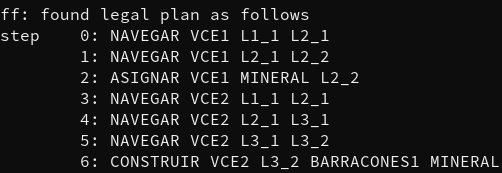
\includegraphics[scale=0.3]{plan1.png}
	\caption{Plan obtenido en el ejercicio 1.}
	\label{plan1}
\end{figure}

\end{multicols}

\section{Ejercicio 2}

Para este ejercicio se nos pide modificar el anterior para que solo se pueda extraer el recurso Gas si se dispone de un nuevo edificio, el Extractor, en un nodo de Gas.

Al ser una modificación del ejercicio anterior solo indicaré los cambios.

\subsection{Dominio:}

\subsubsection{Constantes:}

Se ha añadido una nueva constante para representar el nuevo edificio: Extractor, de tipo tipoEdificio.

\subsubsection{Acciones:}

Se ha modificado la acción Asignar. Ahora recibe un nuevo parámetro ?edi - edificio. Este parámetro lo usaremos para comprobar que si se va a extraer Gas, en la localización existe el edificio dado por parámetro y es un edificio Extractor.

Para comprobar esta nueva precondición usaremos la orden imply, equivalente al operador lógico de la implicación. Este operador es equivalente a realizar la comprobación $\neg a \lor b$. En nuestro caso $a$ será  (asignarNodoRecursoLocalzizacion Gas ?x), de forma que si en la localización no hay un nodo de Gas no tiene porque cumplirse $b$, sin embargo, si es Gas se tiene que cumplir $b$, que será (and (entidadEnLocalizacion ?edi ?x) (esEdificio ?edi Extractor) para comprobar que tenemos el edificio dado en la localización, y ese edificio es de tipo Extractor.

\subsection{Problema:}

\subsubsection{Objetos:}

Ahora será necesario declarar al menos un objeto extractor por si necesita construirse en algún momento.

\subsubsection{Estado inicial:}

El estado inicial será el mismo, solo que añadiendo la inicialización para representar que el extractor.

\subsubsection{Meta:}

El objetivo de este ejercicio es el mismo que el del ejercicio anterior. Debido a que para construir los barracones no es necesario Gas y no se puede comprobar que construye el extractor de forma correcta, he realizado pruebas usando de meta que el objetivo sea estar extrayendo Gas para comprobar que funciona.

\subsection{Solución:}

\begin{multicols}{2}

Tras ejecutarlo con Metric-FF obtenemos:


\begin{figure}[H]
	\centering
	\vspace*{-1cm}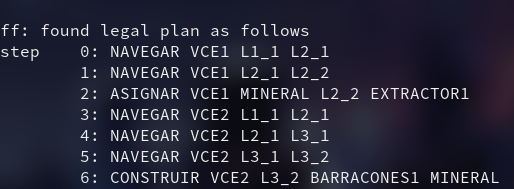
\includegraphics[scale=0.3]{plan2.png}
	\caption{Plan obtenido en el ejercicio 2.}
	\label{plan2}
\end{figure}

\end{multicols}

\begin{multicols}{2}

Y como vemos, al no extraer Gas, no construye el extractor, para comprobar que funciona he realizado una modificación en la meta (la versión entregada tiene la meta pedida en el guión, no esta modificación):


\begin{figure}[H]
	\centering
	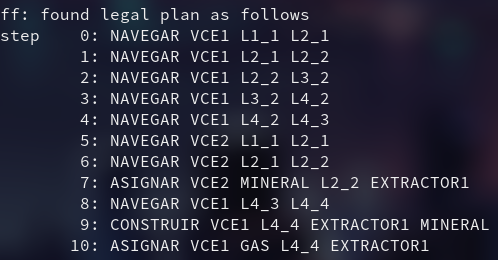
\includegraphics[scale=0.3]{plan2Gas.png}
	\caption{Plan obtenido en el ejercicio 2 con la meta modificada.}
	\label{plan2Gas}
\end{figure}
\end{multicols}

Y podemos ver como antes de extraer Gas es construido el Extractor.

\section{Ejercicio 3}

En este ejercicio tenemos que modificar la acción Construir para tener en cuenta que un edificio puede necesitar varios recursos, así como que solo es necesario marcar el tipo de edificio en el predicado para establecer las necesidades de recursos al construir.

\subsection{Dominio:}

Para este ejercicio solo hay que modificar las acciones y un predicado.

\subsubsection{Predicados:}

Se ha modificado el predicado necesitaRecurso, ahora el primer parámetro es de tipo tipoEdificio, para que solo acepte constantes. En los ejercicios anteriores se hacía con constantes, pero era posible que se usara un objeto de tipo edificio y no las constantes.

\subsubsection{Acciones:}

Modificaré la acción Construir. Ahora solo recibirá tres parámetros, la unidad, la localización y el edificio, en lugar de cuatro, eliminando el parámetro del recurso.

También se ha modificado la precondición, ahora en lugar de comprobar que se necesita el recurso dado y este se está extrayendo, tenemos una estructura forall, en la que comprobaremos para todos los tipoRecurso del dominio, si existe un tipoEdificio tal que el edificio a construir es de dicho tipo, y usando la orden imply, si ese tipo edificio necesita el tipo de recurso este se tiene que estar extrayendo.

\subsection{Problema:}

\subsubsection{Estado inicial:}

En el estado inicial se han añadido predicados para actualizar las necesidades de los edificios, de forma que como dice el guión, el centro de mando necesite tanto mineral como gas para ser construido. Al estar haciendo uso de las constantes desde un principio no ha sido necesario actualizar las necesidades de los edificios que tenemos del ejercicio anterior.

\subsubsection{Meta:}

El objetivo de este ejercicio es el mismo que el de ejercicios anteriores. Debido a que para construir los barracones no comprobamos si se realiza correctamente el construir con varios recursos, he realizado pruebas usando de meta que el objetivo sea construir otro centro de mando (añadido previamente en la sección de objetos y estado inicial para inicializarlo) para comprobar que funciona.

\subsection{Solución:}

\begin{multicols}{2}

Tras ejecutarlo con Metric-FF obtenemos:


\begin{figure}[H]
	\centering
	\vspace*{-1cm}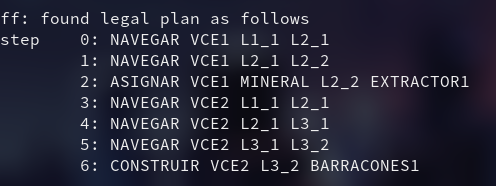
\includegraphics[scale=0.2]{plan3.png}
	\caption{Plan obtenido en el ejercicio 3.}
	\label{plan3}
\end{figure}

\end{multicols}


\begin{multicols}{2}
He realizado una prueba para comprobar que funciona. (la versión entregada tiene la meta pedida en el guión, no esta modificación).

\begin{figure}[H]
	\centering
	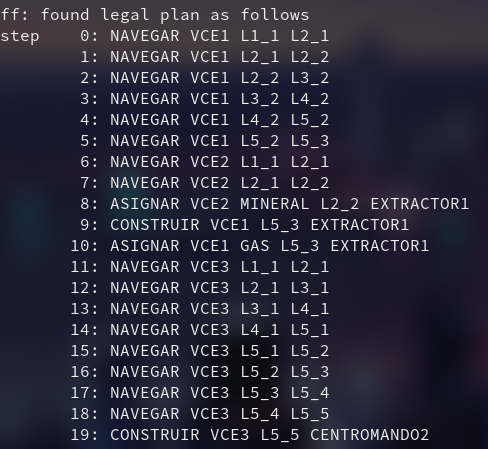
\includegraphics[scale=0.2]{plan3C.png}
	\caption{Plan obtenido en el ejercicio 3 con la meta modificada.}
	\label{plan3C}
\end{figure}



\end{multicols}

\section{Ejercicio 4}

Este ejercicio nos pide añadir una nueva acción Reclutar, así como nuevas unidades, Marines y Segadores. El centro de mando podrá reclutar VCE y los barracones Marines y Segadores.

\subsection{Dominio:}

\subsubsection{Constantes:}

He añadido constantes para representar las dos nuevas unidades.

\subsection{Predicados:}

Se modifica el predicado necesitaRecurso, ahora el primer parámetro es de tipo entidad para poder indicar los recursos necesarios tanto para reclutar unidades como para construir edificios

\subsubsection{Acciones:}

He modificado la acción Asignar y Construir, ya que el guion nos dice que solo pueden extraer recursos y construir los VCE, luego a estas dos acciones le he añadido la precondición de que las unidades que realicen estas acciones sean VCE.


Ahora existirá una nueva acción Reclutar. Como parámetros tiene la unidad a reclutar (?u), el edificio donde se está reclutando (?e) y la localización donde se encuentra el edificio (?x).

Como precondición, no puede existir una localización donde esté la unidad, es decir, la unidad no puede estar ya reclutada, usando el predicado esUnidad en conjunto con la orden imply comprobaremos que tenemos los recursos necesarios. Usando el predicado esEdificio comprobaremos que se reclutan en los edificios correctos, es decir, si el edificio dado es un centro de mando, la unidad ha de ser de tipo VCE, si son unos barracones, de tipo Marine o Segador.

Como efecto, usando el predicado entidadEnLocalización posicionamos la nueva unidad y además marcamos que está libre con unidadLibre.


\subsection{Problema:}

\subsubsection{Objetos:}

Añadimos objetos para representar dos marines y un segador, como nos pide el ejercicio.

\subsubsection{Estado inicial:}

Ahora solo tenemos posicionados un centro de mando y un VCE en el mapa. Además se ha modificado los recursos necesarios y predicados iniciales para representar las necesidades de recursos y tipos de las nuevas unidades.

\subsubsection{Meta:}

Este ejercicio tiene como meta tener dos marines y un segador en posiciones arbitrarias.

\subsection{Solución:}

\begin{multicols}{2}

Tras ejecutar el ejercicio en Metric-FF obtenemos el siguiente plan. Debido a la longitud del plan, en la imagen he eliminado las acciones de navegar por el mapa para que se vea más claro que acciones está realizando.

\begin{figure}[H]
	\centering
	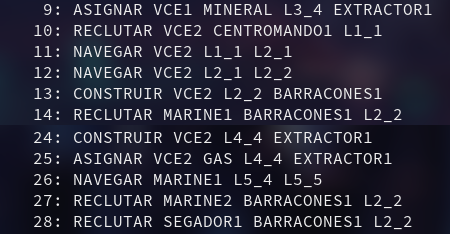
\includegraphics[scale=0.3]{plan4.png}
	\caption{Plan obtenido en el ejercicio 4.}
	\label{plan4}
\end{figure}

\end{multicols}






\section{Ejercicio 5}

En este ejercicio se nos pide añadir un nuevo elemento, las investigaciones, que serán realizadas en el nuevo edificio, la Bahia de Ingeniería. Además para poder reclutar a los Segadores será necesario tener la investigación Impulsor Segador.

\subsection{Dominio:}

\subsubsection{Tipos:}

Para este ejercicio añadimos un tipo nuevo investigación, subtipo de entidad, así como el tipo tipoInvestigacion, subtipo de investigación, para referirnos a las posibles investigaciones.

\subsubsection{Constantes:}

Se ha añadido una constante para representar la investigación ImpulsorSegador, de tipo tipoInvestigacion.

\subsubsection{Predicados:}

Se han añadido dos predicados, esInvestigacion, para enlazar los objetos investigacion con las constantes y (heInvestigado ?inv - investigacion), para representar que ya se ha realizado cierta investigación

\subsubsection{Acciones:}

Se ha modificado la acción Reclutar, ahora si es un segador, además de comprobar que se extraen los recursos necesarios comprueba que se tenga la investigación de tipo ImpulsorSegador.

Se ha añadido la acción Investigar. Como parámetros tiene la investigación a investigar y el edificio donde investigar. Como precondiciones, el edificio a investigar es BahiaIngenieria,  y tiene que existir una localización donde esté (tiene que estar construido). No se tiene que tener investigado la investigación a llevar a cabo, y de forma similar a la forma de construir, comprobamos que se tienen todos los recursos necesarios para la investigación haciendo uso de la orden forall. Como efecto representamos que se ha llevado a cabo la investigación con con el predicado (heInvestigado ?inves).


\subsection{Problema:}

\subsubsection{Objetos:}

En los objetos añadimos tanto el edificio de bahía de ingeniería a construir como la investigación del impulsor.

\subsubsection{Estado inicial:}

En el estado inicial añadimos la inicialización de los nuevos objetos, enlazando la investigación y la bahía con sus respectivas constantes.

\subsubsection{Meta:}

La meta es la misma que en el ejercicio anterior, tener dos marines y un segador en posiciones arbitrarias.

\subsection{Solución:}

\begin{multicols}{2}

Tras lanzar Metric-FF obtenemos el siguiente plan (por la longitud he eliminado las acciones navegar de la imagen, al ser simplemente unidades moviéndose)  :



\begin{figure}[H]
	\centering
	\vspace*{-1cm}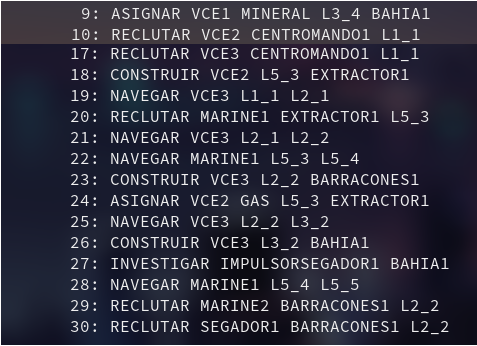
\includegraphics[scale=0.2]{plan5.png}
	\caption{Plan obtenido en el ejercicio 5.}
	\label{plan5}
\end{figure}

\end{multicols}


\section{Ejercicio 6}

Este ejercicio nos pide añadir una nueva función para recolectar recursos. Por cada trabajador asignado a un nodo se incrementa en 25 el recurso cada vez que realicemos la acción extraer, además debemos incluir una acción para desasignar un VCE a un nodo. También tenemos que modificar las acciones construir, reclutar e investigar para tener en cuenta de que ahora se necesita cierto número de recursos dependiendo del edificio, unidad o investigación. También tendremos un nuevo edificio, Deposito. En principio tendremos un límite de 100 para cada recurso, y al construir un deposito aumentaremos en 100 dicho límite para ambos recursos.

\subsection{Dominio:}

\subsubsection{Constantes:}

Añadimos el nuevo edificio Deposito, de tipo tipoEdificio.

\subsubsection{Predicados:}

Eliminamos el predicado neccesitaRecurso, ya que ahora tiene que tener un valor numérico.

\subsubsection{Funciones:}

Se declaran en la sección \texttt{:functions}. Nos servirán para representar valores numéricos en el dominio y problema. El valor inicial lo estableceremos en el problema y lo modificaremos en las acciones, con las ordenes increase y decrease.

Usaremos las siguientes funciones:

\begin{itemize}
	\item (necesitaRecurso ?x - entidad ?r - recurso): Para marcar cuanta cantidad de recurso requiere construir o reclutar una entidad.
	\item (recursoAlmacenado ?tR - tipoRecurso): Para representar la cantidad de recurso que tenemos disponible.
	\item (topeRecurso ?tR - tipoRecurso): Para representar el máximo de recurso que podemos almacenar.
	\item (unidadesExtrayendo ?tipoRecurso - tipoRecurso): Para contar cuantas unidades están extrayendo cierto recurso.
\end{itemize}

\subsubsection{Acciones:}

Se ha modificado la acción Asignar. Ahora como efecto se incrementa en 1 el valor de la función (unidadesExtrayendo ?rec), siendo ?rec el tipo de recurso que se está extrayendo.

Se ha creado la función Desasignar,  dado una unidad, localización y un tipo de recurso, como precondición la unidad no esta libre, esta en la localización y en dicha localización hay un nodo del tipo de recurso, como efecto, la unidad pasa a estar libre, se decrementa en 1 el número de unidades extrayendo el recurso, y si el número de unidades extrayendo llega a cero, marcamos que no estamos extrayendo dicho recurso.

Se han modificado las acciones construir, reclutar e investigar, todas de la misma forma, se comprueba a través de un forall todos los recursos y que para todos los recursos se tiene suficiente tamaño de almacén (esto para hacer la ejecución más rápida, directamente busca construir un Deposito si no se cumple) y suficiente almacenado para construir.

El efecto de estas acciones se ha modificado para restar con la orden decrease el recurso almacenado tanto como necesitaRecurso la entidad reclutada/construida/investigada.

Se ha añadido un efecto en construir, cuando se construye un Deposito se incrementan en 100 los topes de los recursos.

Se ha añadido la acción de Recolectar. Como parámetro recibe el tipo de recurso, sus precondiciones es que se está extrayendo el recurso y tenemos suficiente espacio en los Depositos (el recurso almacenado es menor que el tope). Como acción se incrementa el recurso en 25 por el número de unidades extrayendo el recurso.

\subsection{Problema:}

\subsubsection{Objetos:}

Hemos declarado más unidades y edificios para poder aprovechar al máximo todos los nodos de recursos (aunque al principio solo tengamos el centro de mando y un VCE).

\subsubsection{Estado inicial:}

He actualizado los recursos necesarios para cada entidad conforme a la tabla dada, así como establecido los topes de recursos a los indicados.

\subsubsection{Meta:}

Para este ejercicio tenemos la misma meta, tener dos marines y un segador.

\subsection{Solución:}

\begin{multicols}{2}

Tras ejecutar este ejercicio sobre Metric-FF obtenemos el siguiente plan (debido a la complejidad y longitud del plan solo muestro la parte final, para comprobar que se recolectan los recursos correctamente y se llega a reclutar al segador, la unidad más compleja debido a la necesidad de investigar): 

\begin{figure}[H]
	\centering
	\vspace*{-1cm}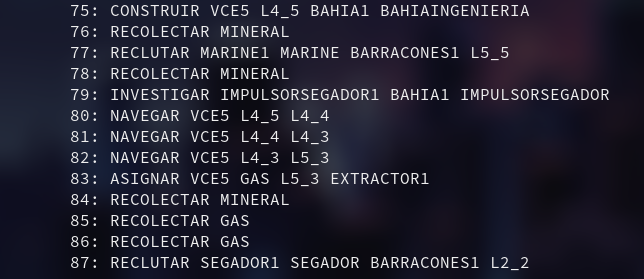
\includegraphics[scale=0.3]{plan6.png}
	\caption{Plan obtenido en el ejercicio 6.}
	\label{plan6}
\end{figure}

\end{multicols}
Cabe destacar que debido a la complejidad que ha tomado este ejercicio, ahora son necesarios unos 10/15 segundos para que el planificador encuentre solución.


\section{Ejercicio 7}


Aunque el ejercicio 7 ha sido retirado de la práctica, cuando se nos aviso de esto ya tenía la codificación lista y funcional, por lo que lo he añadido en la entrega. No realizaré una explicación en profundidad por falta de espacio, pero simplemente se han añadido funciones para saber el tiempo necesario de cada acción y una función para contar el tiempo, cada vez que se realiza una acción se suma el tiempo necesario en el tiempo transcurrido en el fichero de dominio. En el fichero de problema inicializamos los tiempos necesarios y el transcurrido, y en lugar de usar la métrica por defecto uso la métrica \texttt{:metric minimize (tiempoTranscurrido)} para que Metric-FF trate de encontrar el plan con el valor mínimo esta función.


\begin{figure}[H]
	\centering
	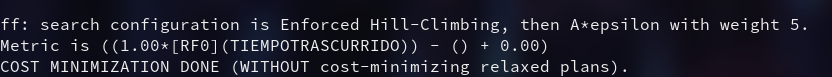
\includegraphics[scale=0.3]{usoMetrica.png}
	\caption{Ejecución de Metric-FF con la nueva métrica.}
	\label{plan7me}
\end{figure}

\begin{figure}[H]
	\centering
	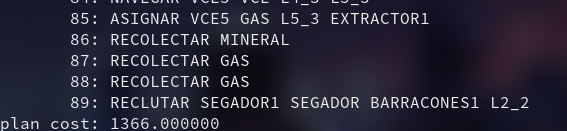
\includegraphics[scale=0.3]{plan7.png}
	\caption{Plan obtenido en el ejercicio 7, coste del tiempo.}
	\label{plan7}
\end{figure}

\end{document}
